
%%%%%%%%%%%%%%%%%%%%%%%%%%%%%%%%%%%%%%%%%%%%%%%%%%%%%%%%%%%%%%%%%%%%%%%
\subsection{Logkorrelation in Cloud-Umgebungen}
%%%%%%%%%%%%%%%%%%%%%%%%%%%%%%%%%%%%%%%%%%%%%%%%%%%%%%%%%%%%%%%%%%%%%%%
\begin{frame}
\frametitle{Cloud}
\framesubtitle{Anforderungen an eine Logkorrelation}

    \begin{block}{cloud - IaaS}
        \begin{itemize}
            \item Stark steigende Systemanzahl (10K+)
            \item In wenigen Sekunden: virtuelles RZ
            \item Dynamisch wachsendes/sinkendes Logaufkommen
            \item Dynamische Kosten
            \item \color{red}{Proprietäre, inkompatible Monitoringsysteme}
            \footnote{IETF-draft: \textit{Syslog Extension for Cloud Using Syslog 
            Structured Data}}
        \end{itemize}
    \end{block}
    \pause
    \begin{block}{Anforderungen Logkorrelation}
        \begin{itemize}
            \item Manuell undurchführbar
            \item Skalierbar (n+1)
            \item Automatisch durchführbar
            \item Minimierung des Speicheraufwandes
        \end{itemize}
    \end{block}

\end{frame}
%%%%%%%%%%%%%%%%%%%%%%%%%%%%%%%%%%%%%%%%%%%%%


\begin{frame}
\frametitle{Prototyp JCorrelat}
\framesubtitle{Schema}


 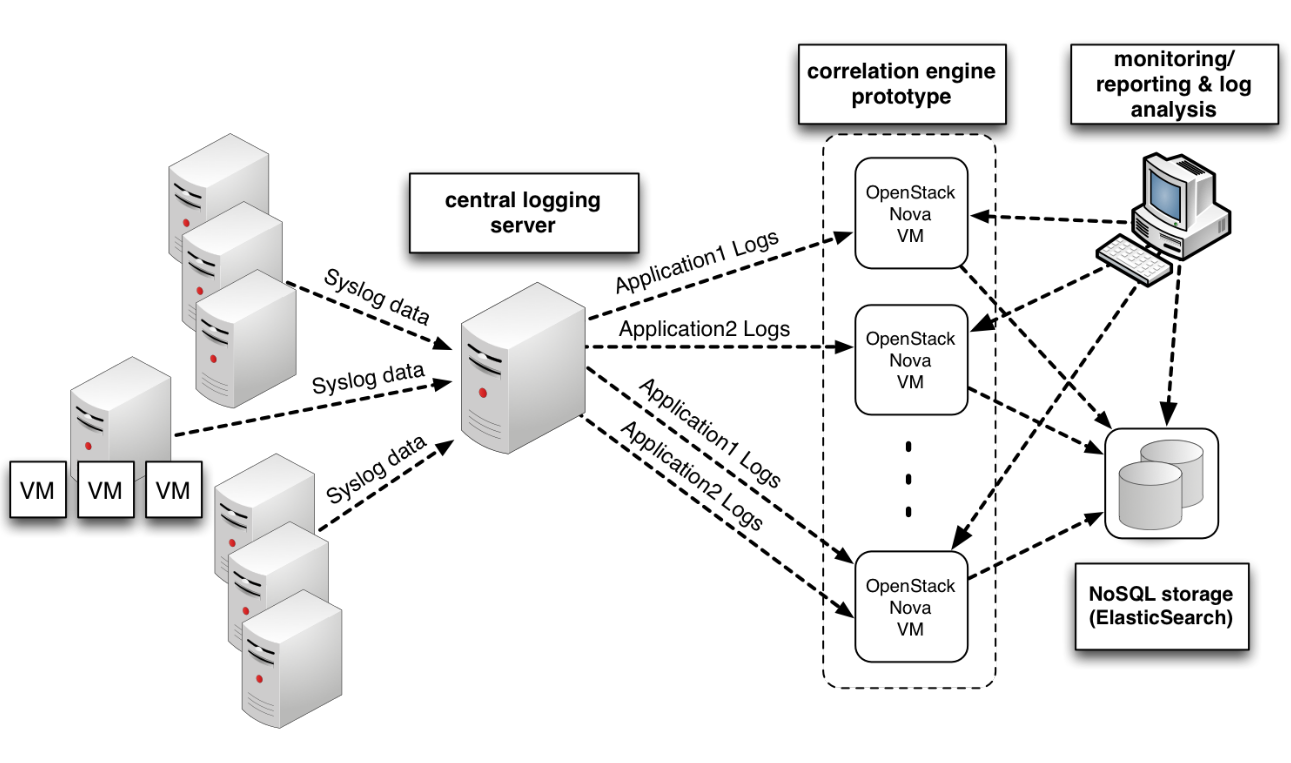
\includegraphics[scale=0.25]{img/schema_correlat-00.png}
\vspace{0.5cm}

\footnoterule
\footnotesize{
    Quelle:
    D.Frisch ,C. Pape, S. Reissmann, and S. Rieger “Correlation and
    Consolidation of Distributed Logging Data in Enterprise Clouds” In International
    Journal on Advances in Internet Technology, vol 7 , 2013, pp. 39–51.}

\end{frame}
%%%%%%%%%%%%%%%%%%%%%%%%%%%%%%%%%%%%%%%%%%%%%

\begin{frame}
\frametitle{Syslog}
\framesubtitle{Aufbau RFC 3164}
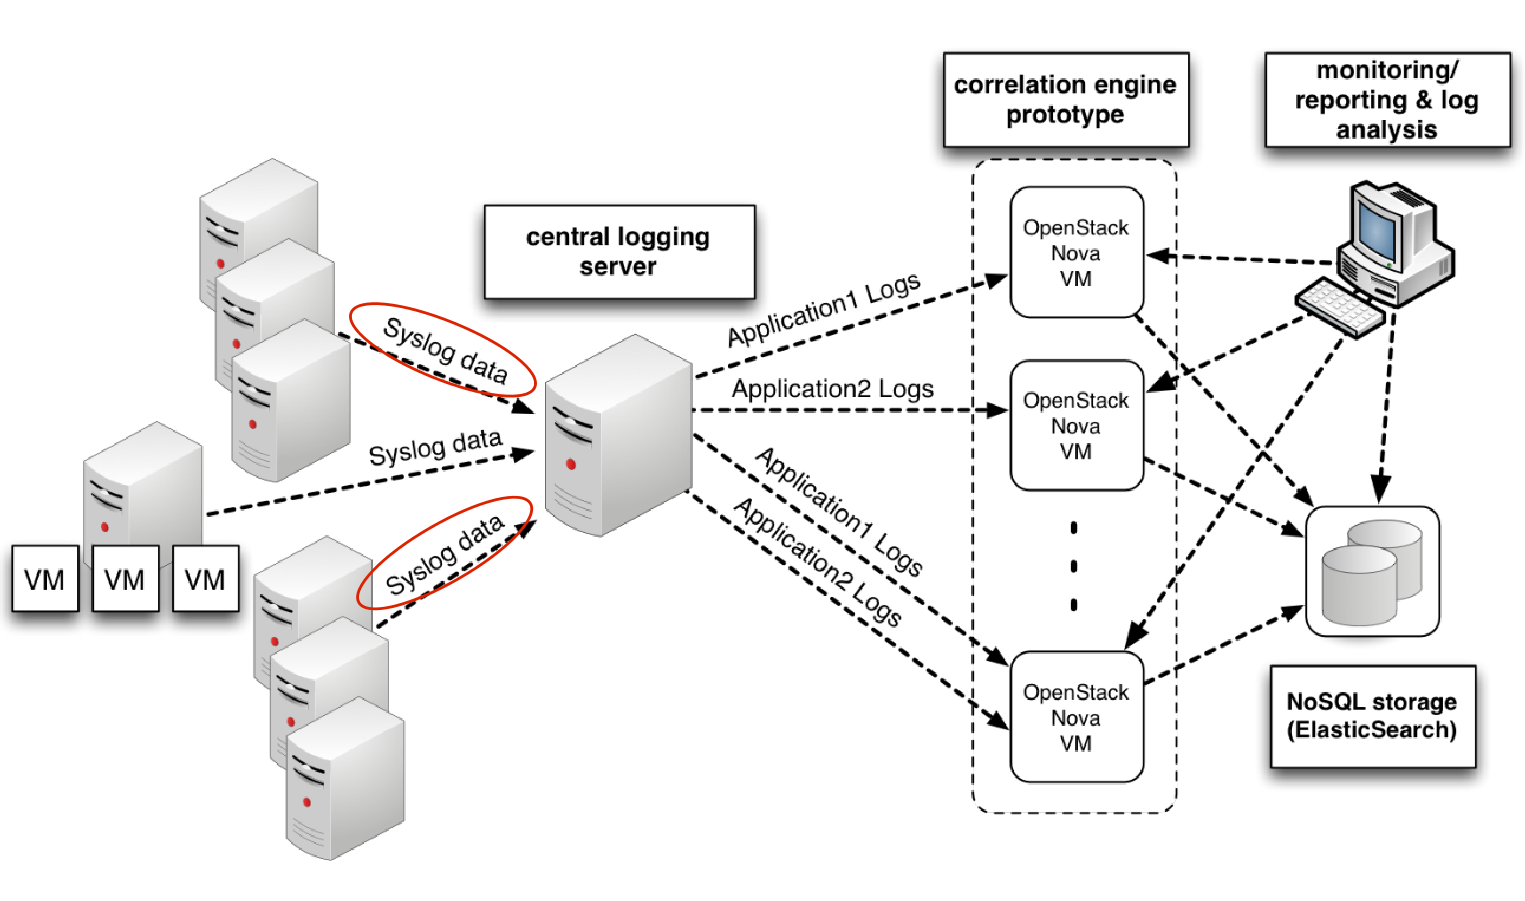
\includegraphics[scale=0.25]{img/schema-correlat-01.png}
\end{frame}


\begin{frame}[fragile]
\frametitle{Syslog}
\framesubtitle{Aufbau RFC 3164}

\begin{center}
\begin{tabular}{|l|c|c|}
  
    \hline 
    \zfA \textbf{Feld}&  \textbf{Inhalt}&
    \textbf{Beispiel}\\ 
    \hline
    \hline
    \zfB\multicolumn{3}{|l|}{PRI}\\
    \hline 
    \zfC facility & $int \in \{0..23\}$  & <\textbf{3}4> (\texttt{sys. daemons}) \\ 
    \hline 
    \zfC severity & $ int \in \{0..7\}$  &<3\textbf{4}> (\texttt{Warning})\\ 
    \hline
    \zfB \multicolumn{3}{|l|}{HEADER}\\
    \hline
    \zfC timestamp &mm dd hh:mm:ss  &\verb|Oct 11 22:14:15|\\ 
    \hline 
    \zfC hostname & string  &\verb|mymachine|\\ 
    \hline 
    \zfB \multicolumn{3}{|l|}{MSG}\\     
    \hline
    \zfC tag &string  &\verb|su:|\\
    \hline
    \zfC content &string&\verb|'su root' failed ...| \\
    \hline
\end{tabular} 
\end{center}

\vspace{0.5cm}
\small{
\begin{verbatim}
<34>Oct 11 22:14:15 mymachine su: 'su root' failed for lonvick
on /dev/pts/8
\end{verbatim}}

\end{frame}
\begin{frame}[fragile]
\frametitle{Syslog + strukturierte Daten}
\framesubtitle{Aufbau RFC 5424}

\centering{ \texttt{RFC5424} Implementiert durch \texttt{syslog-ng} und
    {\color{red}\texttt{rsyslog}}}

\begin{center}
    \begin{tabular}{|l|c|c|}
        
        \hline 
        \zfA \textbf{Feld}&  \textbf{Inhalt}& \textbf{Beispiel}\\ 
        \hline
        \hline
        \zfB \multicolumn{3}{|l|}{HEADER}\\
        \zfC facility & $int \in \{0..23\}$  & <\textbf{16}5> (\texttt{local0}) \\ 
        \hline 
        \zfC severity & $ int \in \{0..7\}$  &<16\textbf{5}> (\texttt{Notice})\\ 
        \hline
        \rowcolor{green} timestamp & \texttt{RFC3339}  &\verb|2003-10-11T22:14:15.003Z|\\ 
        \hline 
        \zfC hostname & string  &\verb|mymachine.example.com|\\ 
        \hline 
        \zfC tag &string  &\verb|evntslog|\\
        \hline
        \zfB \multicolumn{3}{|l|}{MSG}\\     
        \hline
        \rowcolor{green} MSGID& key=value &\verb|ID47| \\
        \hline
        \rowcolor{green} structured data& key=value &\verb|eventID="1011"| \\
        \hline
        \zfC content &string&\verb|An application event log...| \\
        \hline
    \end{tabular} 
\end{center}

\small{
\begin{verbatim}
<165> 2003-10-11T22:14:15.003Z mymachine.example.com evntslog -
ID47 [exampleSDID@32473 iut="3" eventSource= "Application"
eventID="1011"] BOMAn application event log entry...
\end{verbatim}}

\end{frame}

%%%%%%%%%%%%%%%%%%%%%%%%%%%%%%%%%%%%%%%%%%%%%

\begin{frame}
\frametitle{Syslog}
\framesubtitle{Persistente Speicherung und Konsolidierung }
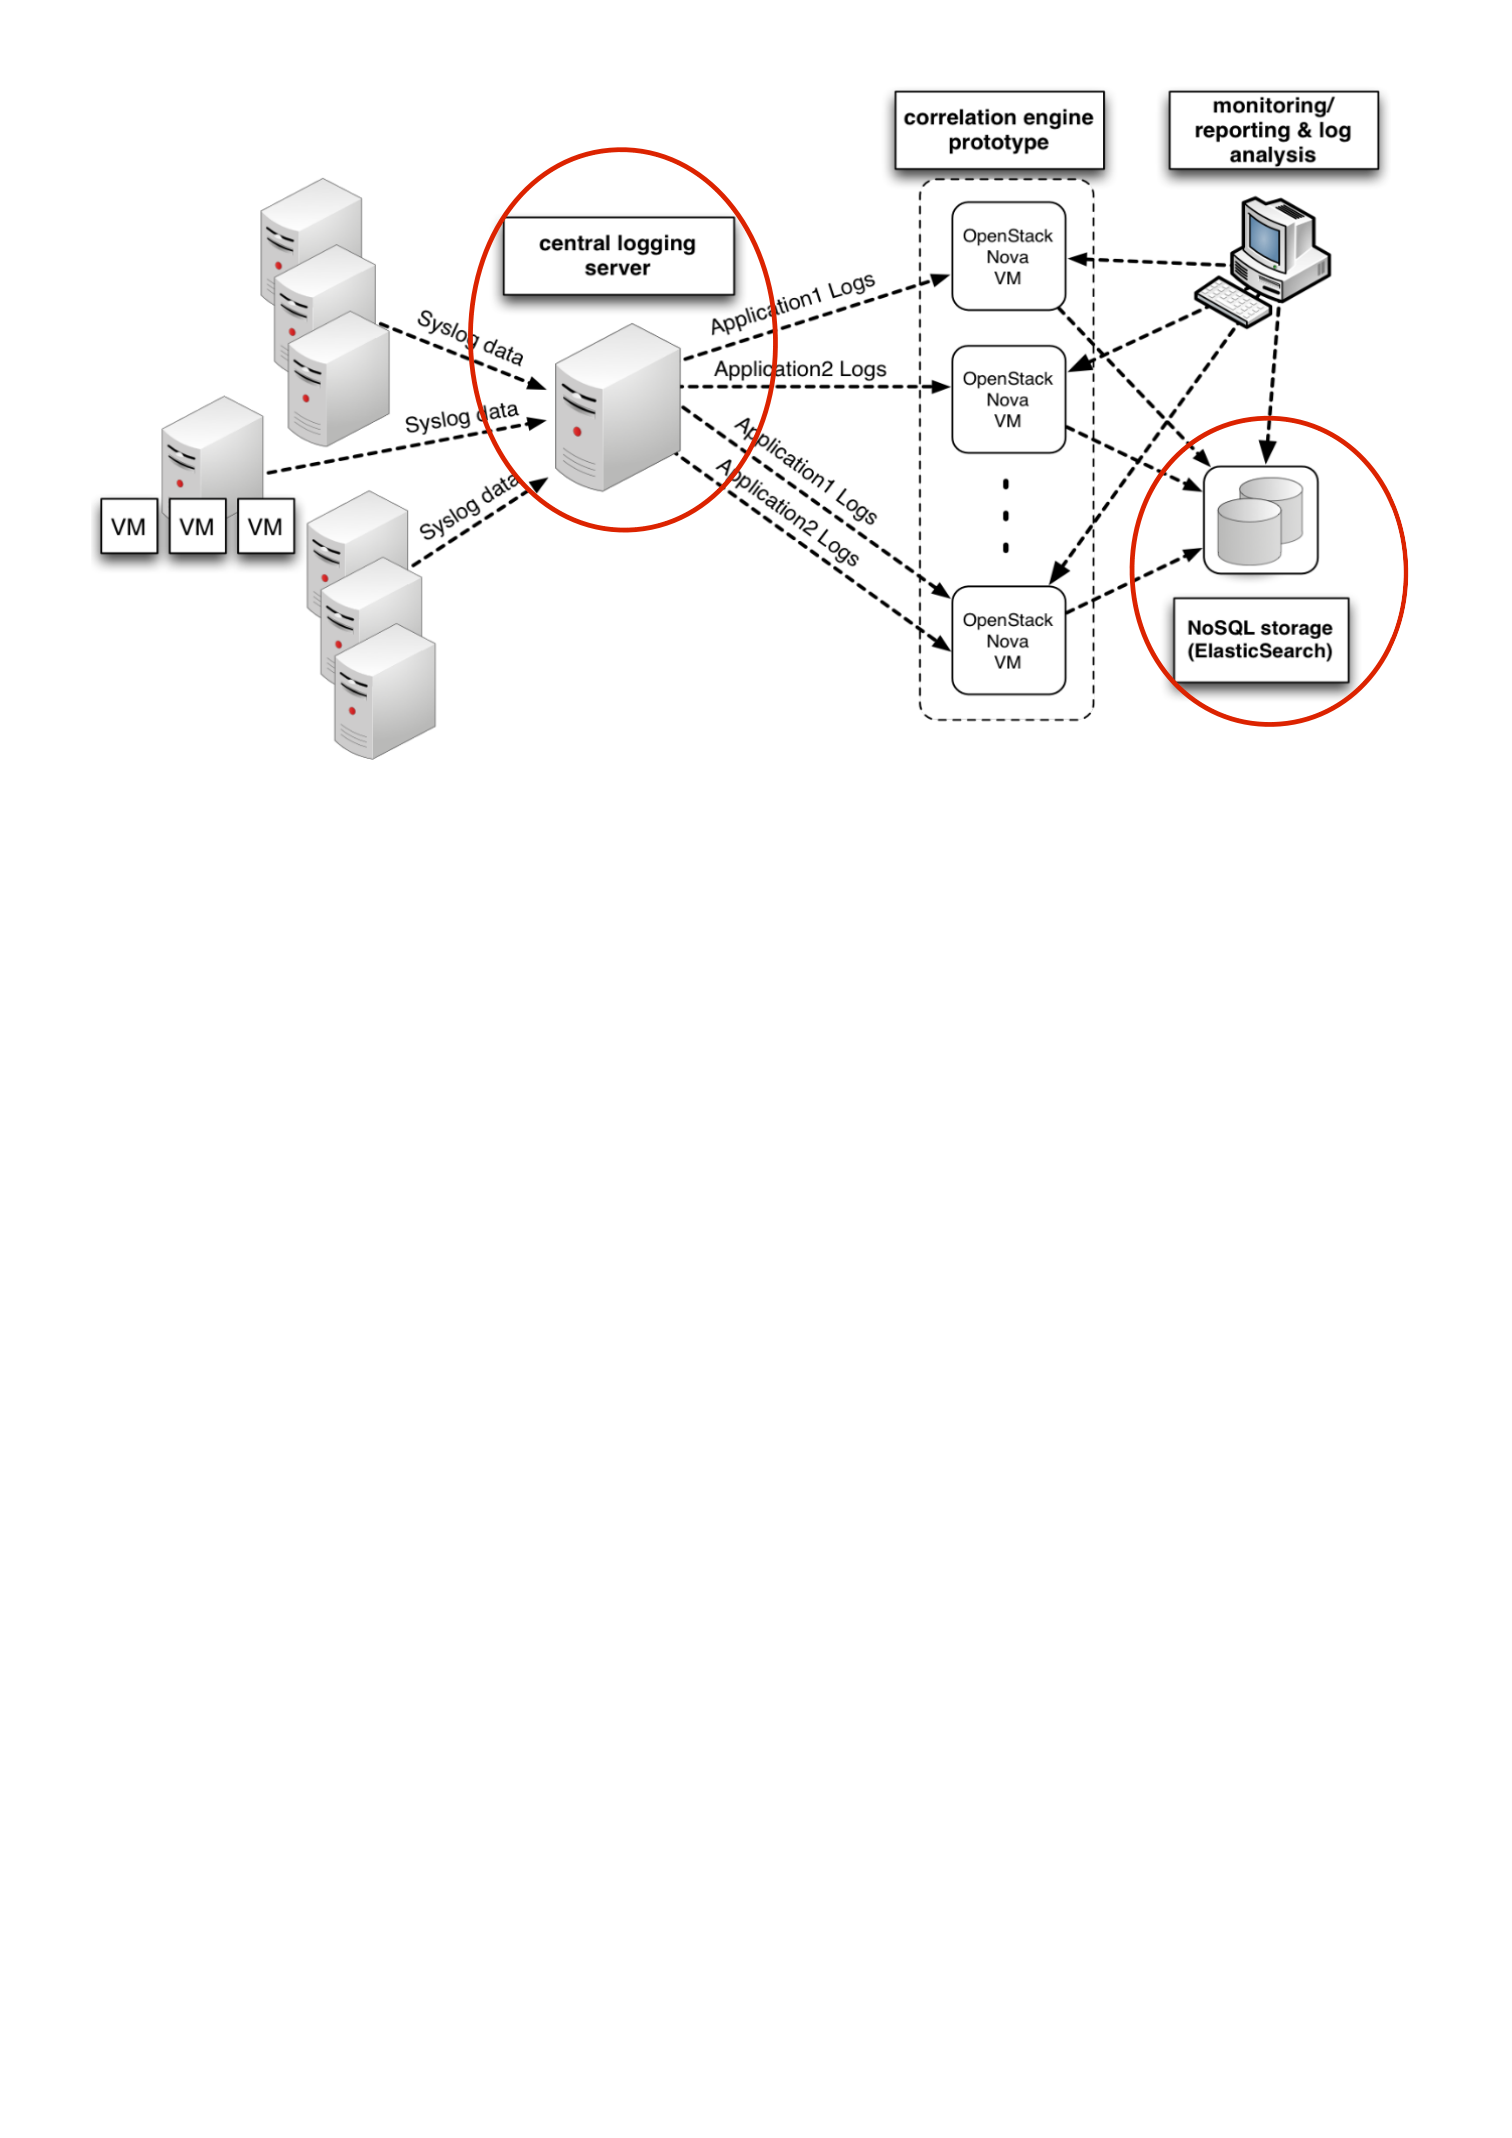
\includegraphics[scale=0.25]{img/schema-correlat-02.png}
\end{frame}


\begin{frame}
\frametitle{Persistente Speicherung}

\pause

\begin{alertblock}{Probleme}
    \begin{itemize}
        \item Menge der anfallenden Daten
        \item Hohe Redundanz der Daten
        \item Durchsuchbarkeit Logdaten
    \end{itemize}
\end{alertblock}

\pause

\begin{alertblock}{Relationale Datenbanken}
    \begin{itemize}
        \item Schema der Daten muss bekannt sein
        \item Schemaänderungen nur schwer möglich
    \end{itemize}
\end{alertblock}
\pause

\begin{exampleblock}{NoSQL (Not only SQL)}
    \begin{itemize}
        \item Kein festes Schema
        \item Wohlformatierte strukturierte Daten (key $\Rightarrow$ val)
        \item Sehr gut skalierbar
    \end{itemize}
\end{exampleblock}
\end{frame}

\begin{frame}
\frametitle{Persistente Speicherung}
\framesubtitle{Überblick über 3 NoSQL-Strategien}
\pause
\begin{block}{\texttt{key $\Rightarrow$ value datastores}}
    \begin{itemize}
        \item Hochperformant (key $\Rightarrow$ BLOB)
        \item Einfache API (\texttt{insert, delete, lookup})
        \item \color{red} Keine Suche in BLOBs
    \end{itemize}
\end{block}
\pause
\begin{block}{\texttt{column-oriented datastores}}
    \begin{itemize}
        \item Verwaltung in Zeilen und Spalten
        \item Skalierung: Auftrennung in \textit{shards}
    \end{itemize}
\end{block}
\pause
\begin{block}{\texttt{document-based datastores}}
    \begin{itemize}
        \item \texttt{document}: Menge an Objekten mit unterschiedlichen Attributen
        \item Skalierung: Aufteilung der Objekte
        \item \color{green} Volltextsuche
    \end{itemize}
\end{block}
\end{frame}

\begin{frame}
\frametitle{Ziel der Korrelation von Logdaten}
\framesubtitle{}

\begin{enumerate}
    \pause
    \item \textbf{Reduktion des Datenaufkommens}
    \begin{itemize}
       \item Konsolidierung
    \end{itemize}
    \pause
    \item \textbf{Identifizierung wesentlicher Informationen}
    \begin{itemize}
        \item Korrelation

    \end{itemize}

\end{enumerate}
\pause
\vspace{0.7cm}
\textbf{Im Folgenden:}\\
\vspace{0.5cm}
Beispielhafte Korrelation anhand einer SSH Brute-Force-Attacke.\\
\vspace{0.5cm}
\textbf{Ziel:} Den {\color{red}\underline{einen}} erfolgreichen Versuch dieser Attacke zu 
identifizieren.
\end{frame}

\begin{frame}[fragile]
\frametitle{Konsolidierung von Logevents}
\framesubtitle{Generierung neuer Lognachrichten }

\begin{block}{\texttt{liblognorm} - Regeln}
\centering Zusammenfassung der gleichen Meldung aus unterschiedlichen Quellen
\end{block}


%{\footnotesize
%\begin{verbatim}
\begin{center}
\begin{minipage}{0.9\textwidth}
\begin{minted}[mathescape,fontsize=\footnotesize,bgcolor=shadecolor]{perl6}
rule=SSHSUCCESS : Accepted password for %user:
word% from %ip:ipv4% port %port : number% %protocol:word%

rule=SSHFAILURE : Failed password for %user:
word% from %ip:ipv4% port %port : number% %protocol:word%

rule=SSHFAILURE : Failed password for invalid user %user:
word% from %ip:ipv4% port %port : number% %protocol:word%

\end{minted}
\end{minipage}
\end{center}
%\end{verbatim}
%}
\end{frame}

\begin{frame}[fragile]
\frametitle{Konsolidierung von Logevents}
\framesubtitle{Serialisierung mittels JSON}

\begin{block}{\texttt{liblognorm} - Normalisierung}
\centering Erstellung strukturierter Daten und Weiterleitung an Korrelierungsinstanz
\end{block}

\begin{center}
    \begin{minipage}{0.7\textwidth}
        \begin{minted}[mathescape,fontsize=\footnotesize,bgcolor=shadecolor]{json}
        
{   "data": {
        "protocol":"ssh2",
        "port" : "54548",
        "ip": "10.0.23.4",
        "user": "root"
    },
    "time":"2014-01-29T16:06:00.000",
    "host":"test.example.com",
    "facility":"auth",
    "severity":"info",
    "program" :"sshd",
    "message":" Failed password for root from
                10.0.23.4 port 54548 ssh2",
    "tags" : ["SSHFAILURE"] }
        \end{minted}
    \end{minipage}
\end{center}
\end{frame}

\begin{frame}
\frametitle{Korrelation}
\framesubtitle{Drools Fusion}
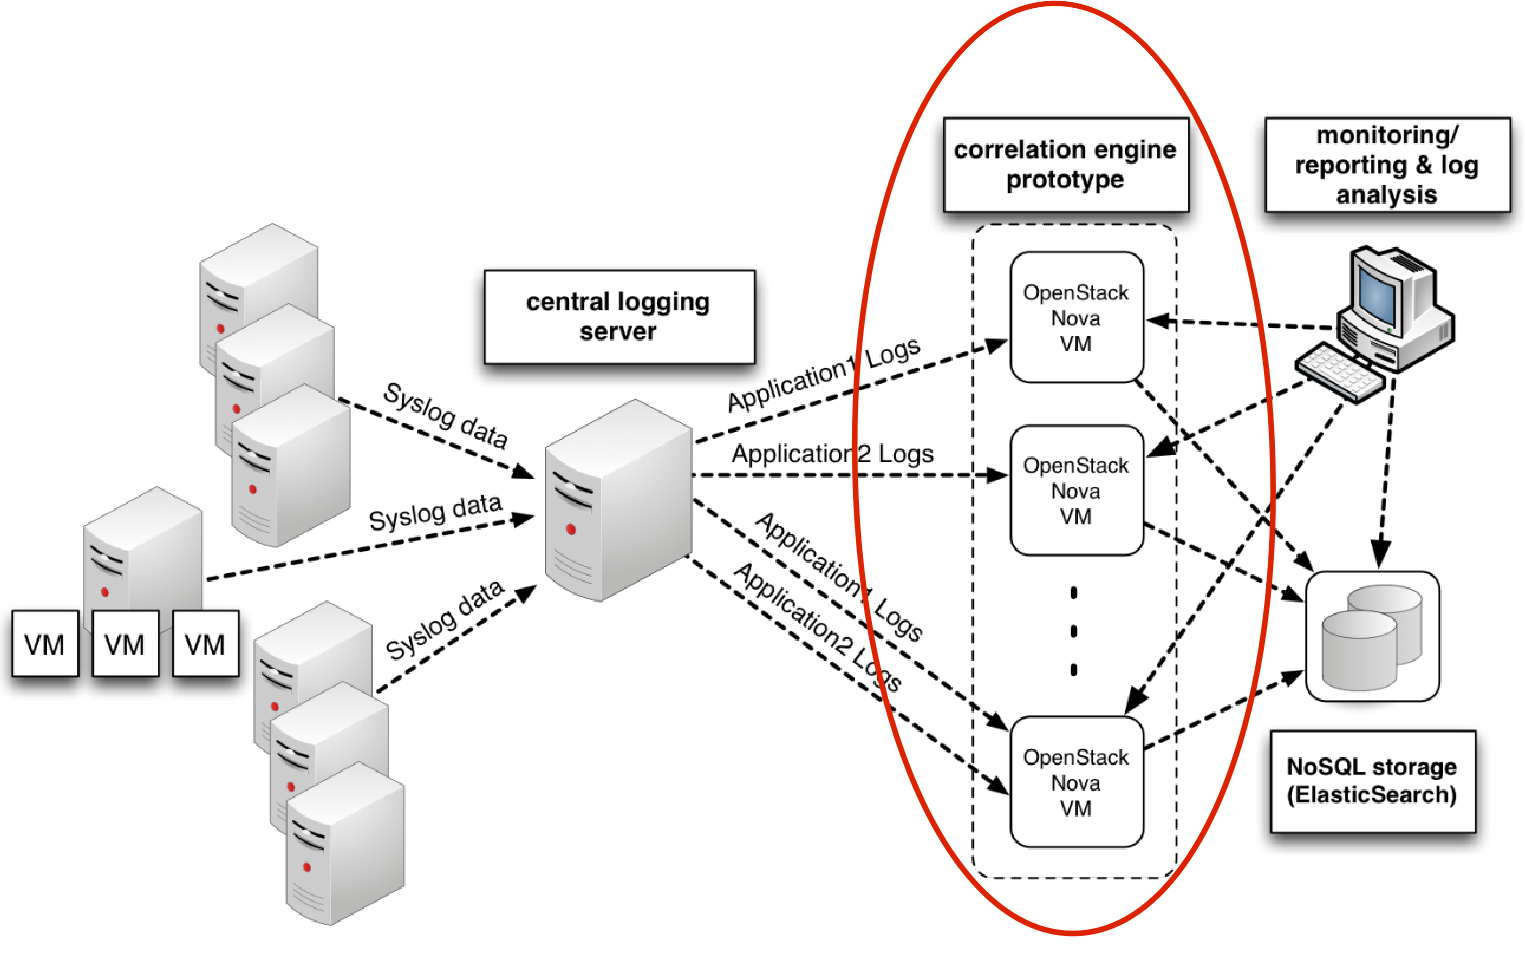
\includegraphics[scale=0.25]{img/schema-correlat-03.png}
\end{frame}


\begin{frame}
\frametitle{Korrelation}
\framesubtitle{Drools Fusion}
\begin{block}{\centering Drools-Fusion}
    \begin{itemize}
        \item Complex Event Processing (CEP) Engine
        \item Regeln basieren auf AL
        \item Zeitliche Schlussfolgerungen
        \item Datenbestand: in-memory-engine
    \end{itemize}
\end{block}

\begin{center}
    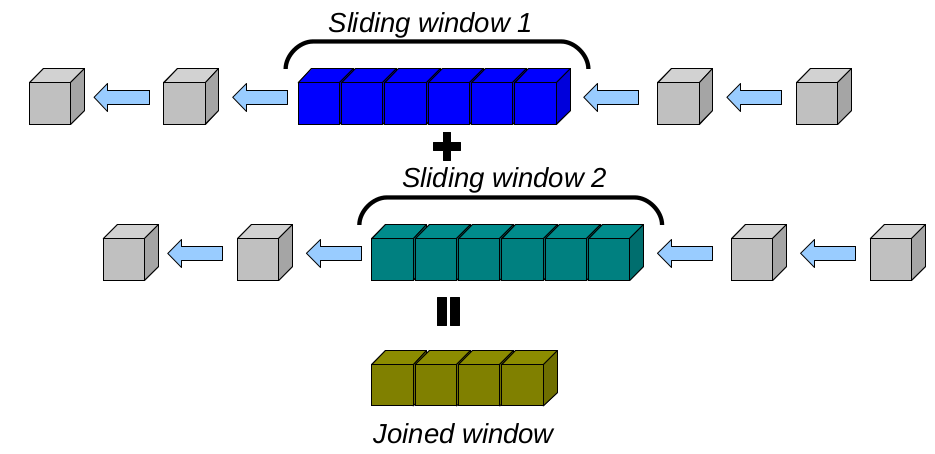
\includegraphics[scale=0.26]{img/drools-slide-00.png}
\end{center}
\vspace{0.3cm}
\footnoterule
\footnotesize{
    Quelle:      Tihomir Surdilovic, RedHat (
\href{https://www.slideshare.net/tsurdilovic/jboss-drools-and-drools-fusion-cep-making-business-rules-react-to-rte}{Slideshare})}

\end{frame}
\begin{frame}[fragile]
\frametitle{Korrelation}
\framesubtitle{Regel 1: \texttt{SSH brute-force attempt}}

\begin{center}
    \begin{minipage}{0.7\textwidth}
        \begin{minted}[mathescape,fontsize=\tiny,bgcolor=shadecolor]{java}
        rule "SSH brute-force attempt"
        no-loop
        when
            Message (   $host:host,
                        $user:data["user"])
            $atts: CopyOnWriteArrayList(size >= 10)
                from collect(
                    Message(    tags contains"SSHFAILURE",
                                host == $host,
                                data["user" ] == $user)
                    over window : time (1m))
        then
            Message last = (Message) $atts.get($atts.size( )-1) ;
        
            for (Object f: $atts) {
                retract ( f ) ;
        }
        
            insert (messageFactory(last)
                . setTime(last.getTime( ))
                . setSeverity(Message.Severity.WARNING)
                . setFacility(Message.Facility.SECURITY)
                . setMessage("SSH brute-force attack" +
                    "for @{data.user} from @{data.ip}")
                . addTag ("BRUTEFORCE")
                . message( )) ;
        end        
        
        \end{minted}
    \end{minipage}
\end{center}

\end{frame}

\begin{frame}[fragile]
\frametitle{Korrelation}
\framesubtitle{Regel 2: \texttt{Successful SSH brute-force attack}}

\begin{itemize}
    \item betrachtet werden: Syslog-tags 
    \item Trifft zu: wenn während einer Brute-Force-Attacke Login gelingt
    \item   \texttt{SSHSUCCESS} innerhalb von 10s nach \texttt{SSHFAILURE} \textbf{und}
            \texttt{BRUTEFORCE} \textbf{und} gleicher \texttt{host}, \texttt{user}
\end{itemize}


\begin{center}
    \begin{minipage}{0.7\textwidth}
        \begin{minted}[mathescape,fontsize=\tiny,bgcolor=shadecolor]{java}
       rule "Successful SSH brute-force attack"
       no-loop
       when
            $ att: Message (    tags contains "SSHFAILURE",
                                tags contains "BRUTEFORCE",
                                $host: host ,
                                $user: data ["user"])
            $ suc: Message (    host == $host,
                                data ["user" ] == $user,
                                tags contains "SSHSUCCESS",
                                this finishes[10 s] $att)
       then
            $att.addTag("INCIDENT");
            $att.setSeverity(Severity.EMERGENCY);
            $att.setMessage($att.getMessage( ) + "[bruteforce]");
       update ($att);
       end
        
        \end{minted}
    \end{minipage}
\end{center}

\end{frame}

\begin{frame}
\frametitle{Korrelation}
\framesubtitle{}

\begin{itemize}
    \item Erzeugung neuer Syslog-Nachrichten durch Regeln
    \item Setzen unterschiedlicher \texttt{severity} (\texttt{Warning}: 4; 
    \texttt{Emergency}: 0)
    \item Auswertung über Visualisierung, \texttt{SNMP-trap}, \texttt{check\_drools}
\end{itemize}

\begin{center}
    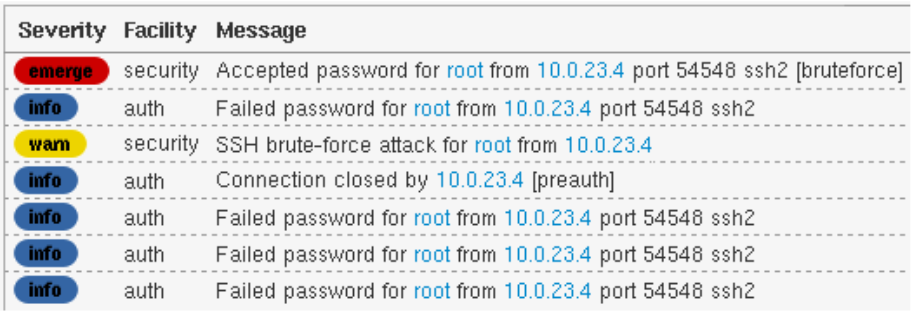
\includegraphics[scale=0.40]{img/correlat-ui.png}
\end{center}

\textbf{Forschungsziel}: \texttt{jCorrelat} soll \textit{correlation template engine} 
werden.

\end{frame}


\begin{frame}
\frametitle{Korrelation}
\framesubtitle{Performance- und Skalierungsbetrachtung}

\begin{center}
    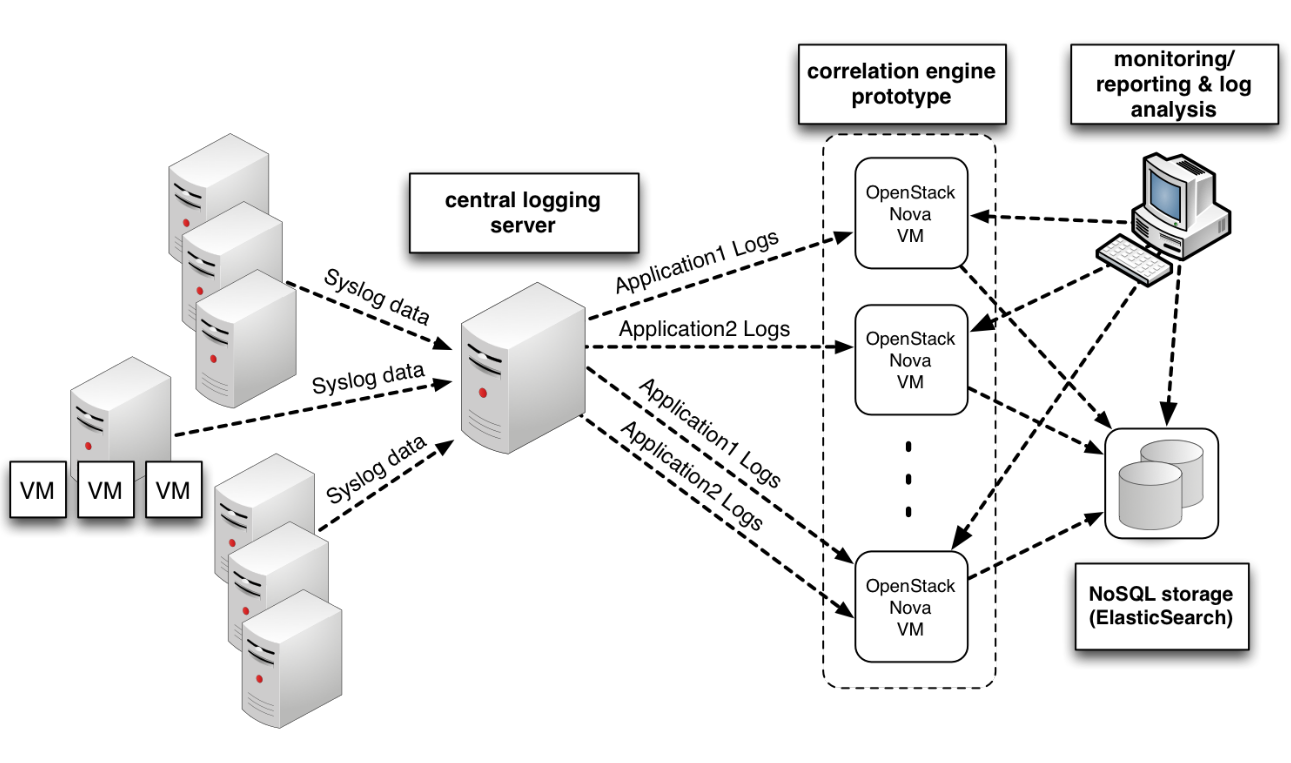
\includegraphics[scale=0.3]{img/schema_correlat-00.png}
\end{center}

\end{frame}


\begin{frame}
\frametitle{Korrelation}
\framesubtitle{Performance- und Skalierungsbetrachtung}

\begin{center}
    \textbf{Benchmark}
    
    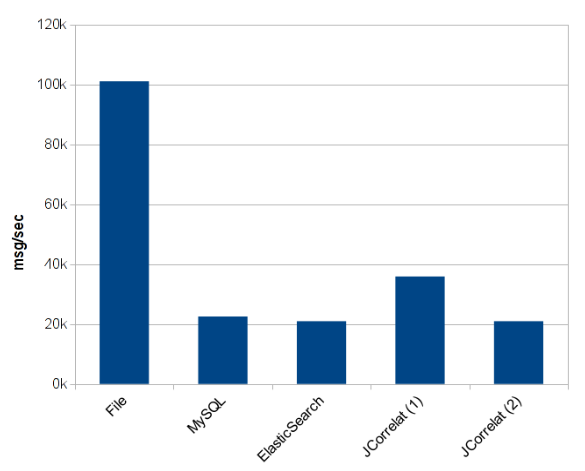
\includegraphics[scale=0.4]{img/benchmark.png}
    
    \color{red}\textbf{Limitierender Faktor}: \textit{in-memory-engine}
\end{center}
\end{frame}


\begin{frame}
\frametitle{Korrelation}
\framesubtitle{Performance- und Skalierungsbetrachtung}

\begin{center}
    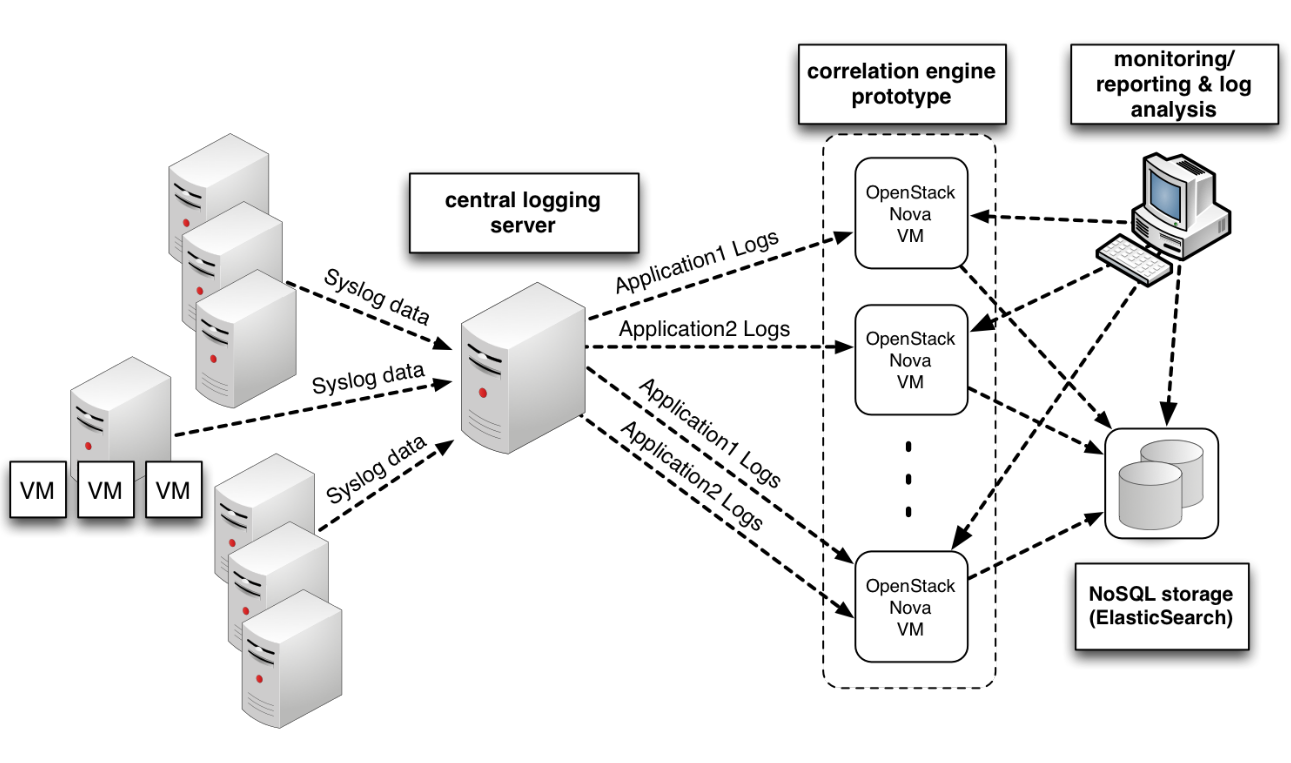
\includegraphics[scale=0.3]{img/schema_correlat-00.png}
\end{center}

\end{frame}